\chapter{Resutls and Evaluation}\label{ch: results and eval}
In this chapter we present our experimental results and their corresponding evaluation. Our experiment was built to evaluation whether DC Transformation helps improve model performance in univariate time series forecasting. Our experiment covers hourly, daily, and weekly frequencies and the results are investigated separately based on the performance metrics we addressed in Section \ref{subsec: performance metrics}.

We start by showing some summary statistics of the agents in Table \ref{tbl: hourly stats}, \ref{tbl: daily stats} and \ref{tbl: weekly stats}. For a model `M', agent using model `M' without DC Transformation is named `M\_raw' and agent using model `M' with DC Transformation is named `M\_tran'. The Tables show that agents with or without DCT do not differ a lot in performance.

\begin{center}
    \begin{table}
        \resizebox{\columnwidth}{!}{\begin{tabular}{|l|r r r r r r|}
            \hline
            {} & Avg. SMAPE & Std. SMAPE & Avg. rank & Std. rank & 90\% rank interval & frac best \\
            \hline\hline
            EN\_raw    &   0.041144 &   0.010202 &         9.95 &        0.218 &           (9.822, 10.078) &       0.0 \\
            EN\_tran   &   0.029771 &   0.006564 &         8.95 &        0.525 &            (8.822, 9.078) &       0.0 \\
            \hline
            ETS\_raw   &   0.017082 &   0.007781 &        5.236 &        1.477 &            (5.108, 5.364) &       0.0 \\
            ETS\_tran  &    0.01727 &   0.006678 &        5.686 &        1.063 &            (5.558, 5.814) &       0.0 \\
            \hline
            LSVR\_raw  &   0.003148 &   0.004825 &        1.243 &        0.445 &            (1.115, 1.371) &     0.764 \\
            LSVR\_tran &   0.017249 &   0.005926 &          5.9 &        1.289 &            (5.772, 6.028) &       0.0 \\
            \hline
            MLP\_raw   &   0.008819 &   0.006091 &        3.057 &         0.41 &            (2.929, 3.185) &       0.0 \\
            MLP\_tran  &   0.019317 &   0.006434 &        7.271 &        1.212 &            (7.143, 7.399) &       0.0 \\
            \hline
            RF\_raw    &    0.00284 &   0.002112 &        1.764 &        0.424 &            (1.636, 1.892) &     0.236 \\
            RF\_tran   &   0.017274 &   0.005028 &        5.921 &        1.358 &            (5.793, 6.049) &       0.0 \\
            \hline
        \end{tabular}}
        \caption{Summary statistics of all agents on hourly unknown domain time series}
        {\raggedright \footnotesize The dataset consists of $140$ time series. Average length of the time series is $1008$. \par}
        \label{tbl: hourly stats}
    \end{table}
\end{center}

\begin{center}
    \begin{table}
        \resizebox{\columnwidth}{!}{\begin{tabular}{|l|r r r r r r|}
            \hline
            {} & Avg. SMAPE & Std. SMAPE & Avg. rank & Std. rank & 90\% rank interval & frac best \\
            \hline\hline
            EN\_raw    &   0.009179 &    0.00977 &        2.357 &        1.285 &            (2.258, 2.456) &     0.266 \\
            EN\_tran   &   0.009186 &   0.009906 &        2.317 &        1.267 &            (2.218, 2.416) &     0.298 \\
            \hline
            ETS\_raw   &   0.009236 &   0.010134 &        3.206 &         1.57 &            (3.107, 3.305) &     0.175 \\
            ETS\_tran  &   0.009377 &   0.010207 &        4.135 &        1.941 &            (4.036, 4.234) &     0.123 \\
            \hline
            LSVR\_raw  &   0.009059 &   0.007686 &        3.548 &        1.924 &            (3.449, 3.647) &     0.298 \\
            LSVR\_tran &   0.009997 &     0.0107 &        7.302 &        1.326 &            (7.203, 7.401) &     0.004 \\
            \hline
            MLP\_raw   &   0.009934 &   0.008717 &        6.948 &        1.802 &            (6.849, 7.047) &     0.024 \\
            MLP\_tran  &    0.01097 &   0.010123 &        9.115 &        1.109 &            (9.016, 9.214) &       0.0 \\
            \hline
            RF\_raw    &   0.009471 &   0.008224 &        5.968 &        1.898 &            (5.869, 6.067) &     0.075 \\
            RF\_tran   &   0.010889 &   0.010496 &        9.179 &        1.163 &             (9.08, 9.278) &       0.0 \\
            \hline
        \end{tabular}}
        \caption{Summary statistics of all agents on daily time series}
        {\raggedright \footnotesize The dataset consists of $252$ time series including micro, macro and financial domain. Average length of the time series is $1179.99$. \par}
        \label{tbl: daily stats}
    \end{table}
\end{center}

\begin{center}
    \begin{table}
        \resizebox{\columnwidth}{!}{\begin{tabular}{|l|r r r r r r|}
            \hline
            {} & Avg. SMAPE & Std. SMAPE & Avg. rank & Std. rank & 90\% rank interval & frac best \\
            \hline\hline
            EN\_raw    &    0.02091 &   0.024271 &          4.0 &        1.954 &            (3.753, 4.247) &     0.121 \\
            EN\_tran   &   0.020935 &   0.024349 &        4.167 &        1.919 &             (3.92, 4.414) &     0.106 \\
            \hline
            ETS\_raw   &   0.020979 &   0.024556 &        4.727 &        2.042 &             (4.48, 4.974) &     0.061 \\
            ETS\_tran  &   0.021029 &    0.02474 &        5.167 &        2.086 &             (4.92, 5.414) &      0.03 \\
            \hline
            LSVR\_raw  &   0.019724 &   0.022382 &        3.091 &        2.227 &            (2.844, 3.338) &     0.348 \\
            LSVR\_tran &   0.022205 &   0.024924 &        7.318 &         2.14 &            (7.071, 7.565) &     0.015 \\
            \hline
            MLP\_raw   &   0.021029 &   0.023338 &        5.667 &        2.749 &             (5.42, 5.914) &      0.03 \\
            MLP\_tran  &   0.022734 &   0.024506 &        8.152 &        2.251 &            (7.905, 8.399) &       0.0 \\
            \hline
            RF\_raw    &   0.020129 &   0.022872 &        3.667 &        2.809 &             (3.42, 3.914) &     0.348 \\
            RF\_tran   &    0.02314 &   0.026118 &        8.091 &        2.598 &            (7.844, 8.338) &     0.045 \\
            \hline
        \end{tabular}}
        \caption{Summary statistics of all agents on weekly financial time series}
        {\raggedright \footnotesize The dataset consists of $66$ time series. Average length of the time series is $1260.70$. \par}
        \label{tbl: weekly stats}
    \end{table}
\end{center}

\begin{figure}
    \centering
    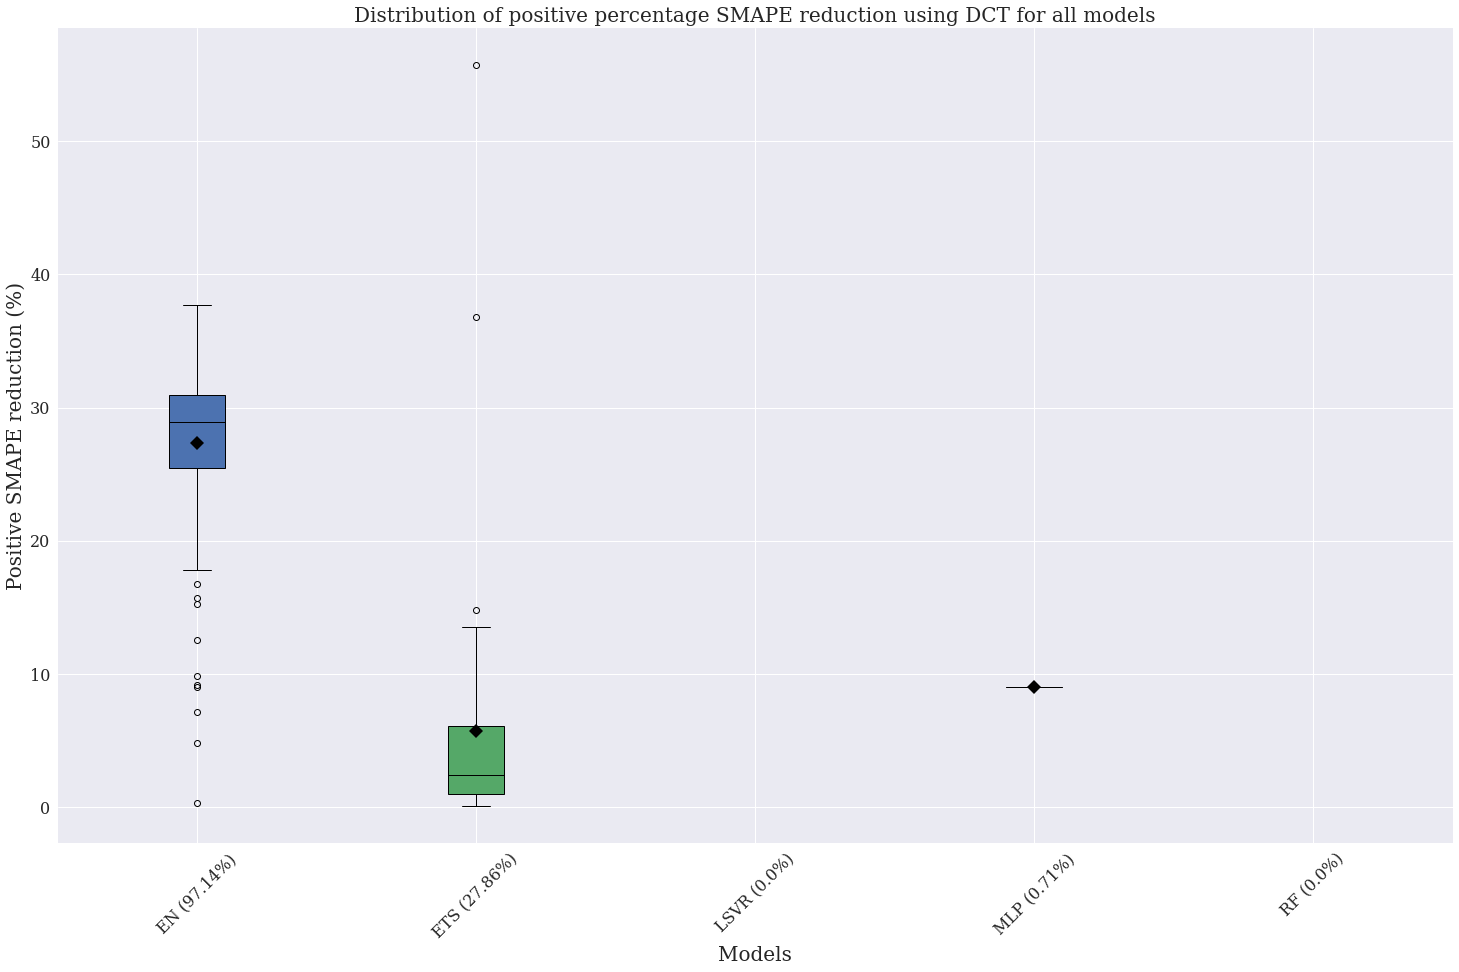
\includegraphics[width=\columnwidth]{hourly_smape_reduce_box_positive}
    \caption{Distribution of positive SMAPE reductions (\%) using DCT}
    {\raggedright \footnotesize The dataset used for this graph consists of $140$ hourly time series in unknown domain. The boxplots are the distributions of positive SMAPE reductions (in percentage) using DC Transformation for each models. The dimons are the mean of the corresponding distribution. The number next to the x-labels are the ratio of DCT giving positve SMAPE reductions out of $140$ time series tested.\par}
    \label{fig: hourly positive smape reduce box}
\end{figure}

\begin{figure}
    \centering
    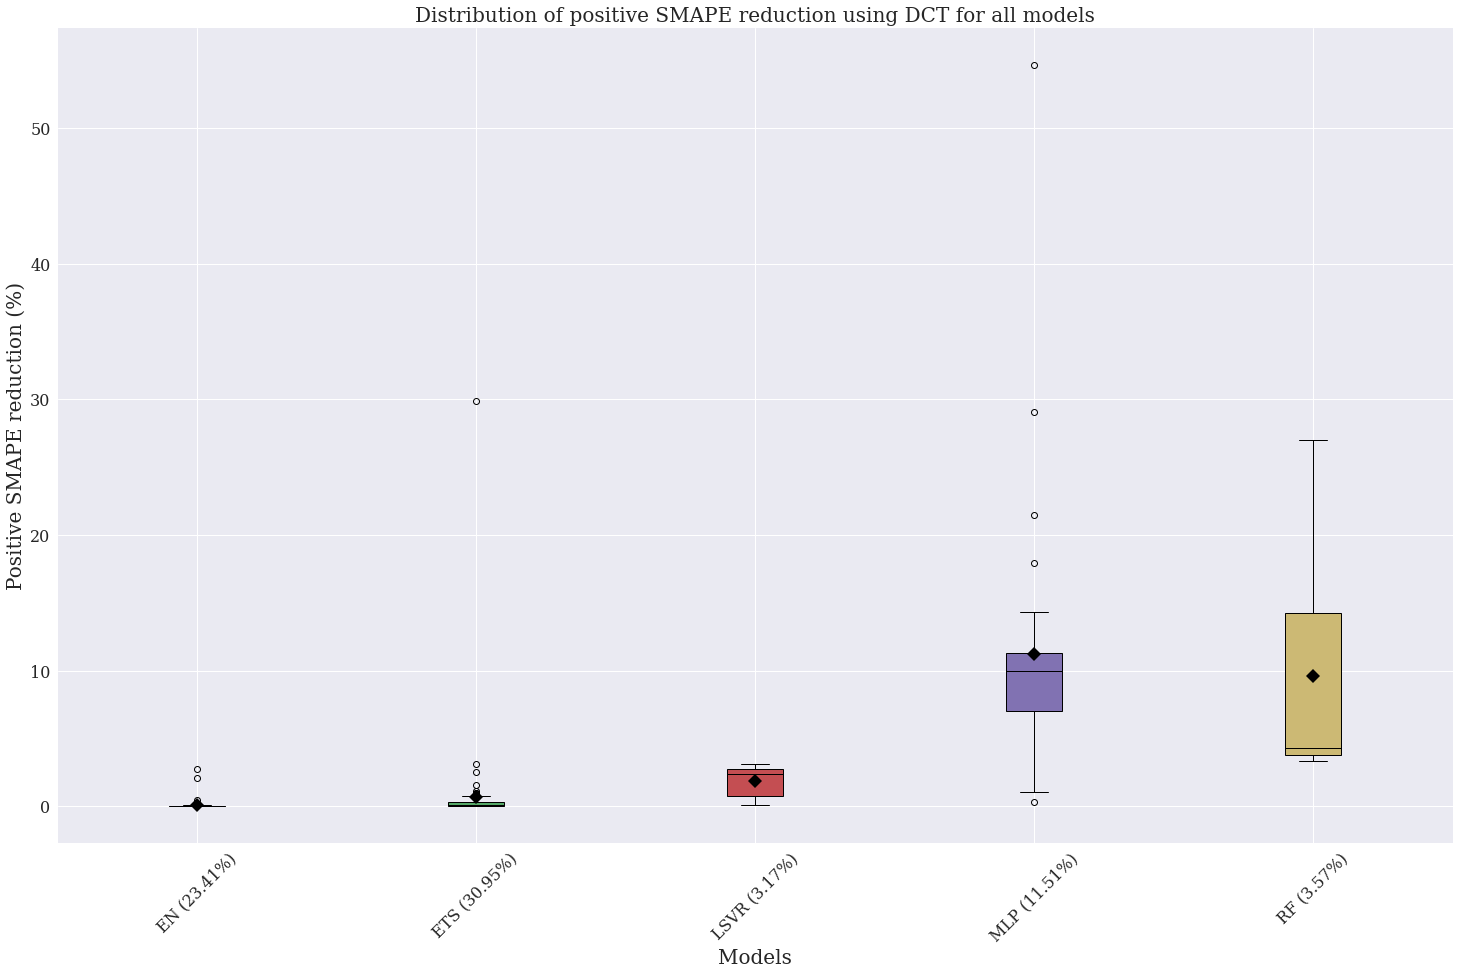
\includegraphics[width=\columnwidth]{daily_smape_reduce_box_positive}
    \caption{Distribution of positive SMAPE reductions (\%) using DCT}
    {\raggedright \footnotesize The dataset used for this graph consists of $252$ daily time series in micro, macro and financial domain. The boxplots are the distributions of positive SMAPE reductions (in percentage) using DC Transformation for each models. The dimons are the mean of the corresponding distribution. The number next to the x-labels are the ratio of DCT giving positve SMAPE reductions out of $252$ time series tested.\par}
    \label{fig: daily positive smape reduce box}
\end{figure}

\begin{figure}
    \centering
    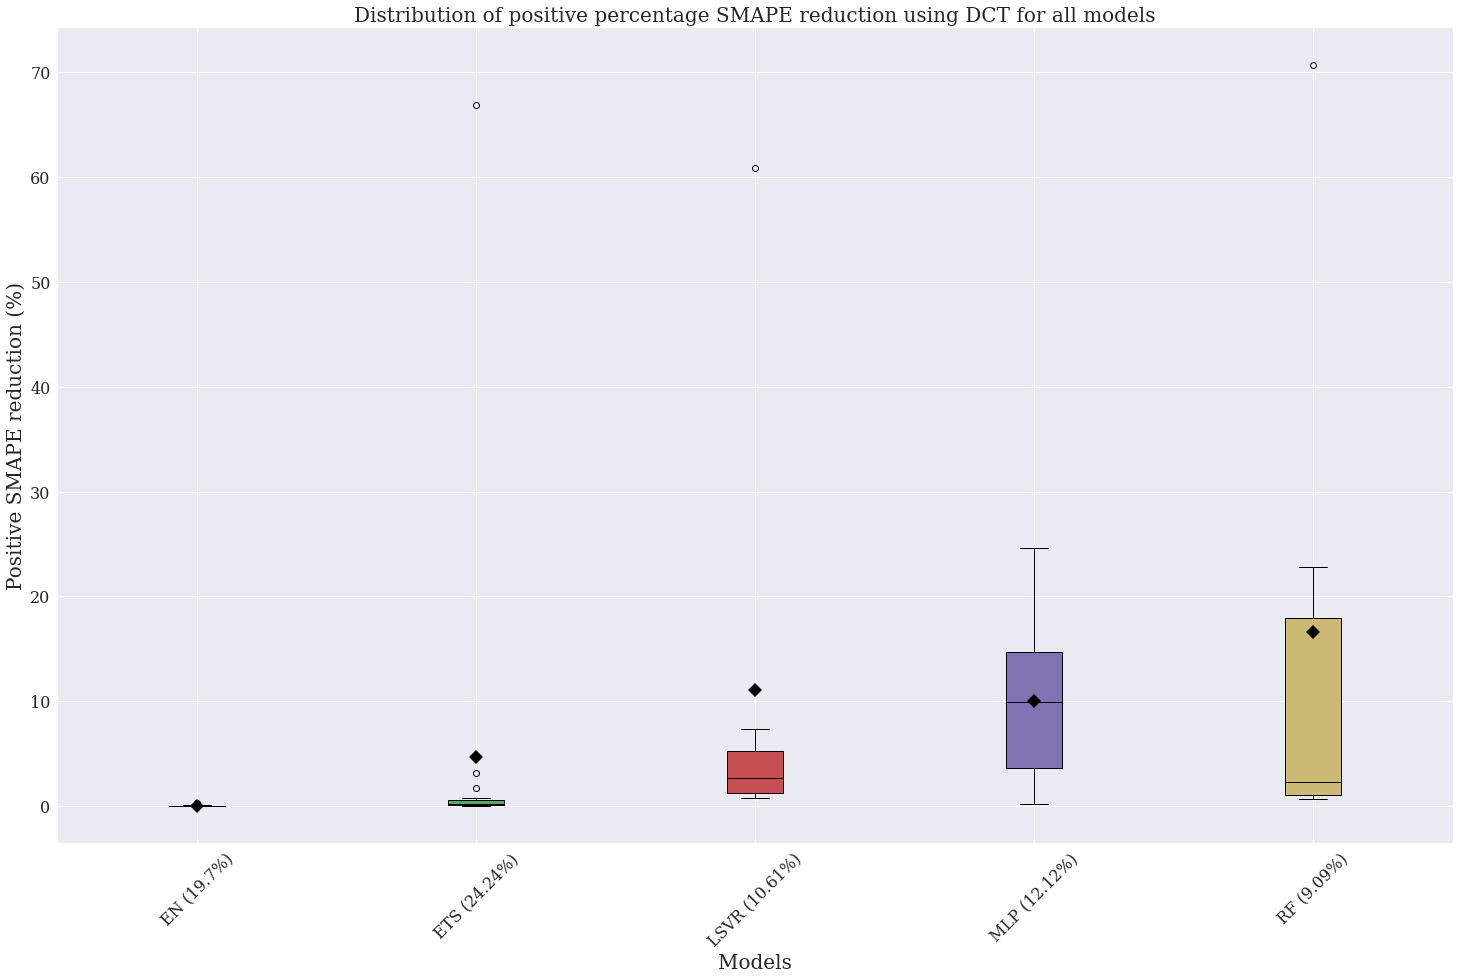
\includegraphics[width=\columnwidth]{weekly_smape_reduce_box_positive}
    \caption{Distribution of positive SMAPE reductions (\%) using DCT}
    {\raggedright \footnotesize The dataset used for this graph consists of $66$ weekly time series in financial domain. The boxplots are the distributions of positive SMAPE reductions (in percentage) using DC Transformation for each models. The dimons are the mean of the corresponding distribution. The number next to the x-labels are the ratio of DCT giving positve SMAPE reductions out of $66$ time series tested.\par}
    \label{fig: weekly positive smape reduce box}
\end{figure}




\begin{center}
    \begin{table}
        \resizebox{\columnwidth}{!}{\begin{tabular}{|l|r r r r r|}
            \hline
            {} & Avg. \% reduction & Std. \% reduction & + reduction ratio & Avg. + \% reduction & Std. + \% reduction \\
            \hline\hline
            EN   &           26.55 &            7.72 &              97.14 &             27.33 &              6.33 \\
            ETS  &           -3.09 &            9.02 &              27.86 &              5.75 &             10.30 \\
            LSVR &         -598.10 &          211.77 &               0.00 &               NaN &               NaN \\
            MLP  &         -135.48 &           46.83 &               0.71 &              9.02 &              0.00 \\
            RF   &         -548.46 &          161.49 &               0.00 &               NaN &               NaN \\
            \hline
        \end{tabular}}
        \caption{Statistics of SMAPE reduction (\%) using DCT (hourly unknown domain)}
        {\raggedright \footnotesize This table shows the statistics of SMAPE reduction (in percentage) using DC Transformation. The dataset used consists of $140$ hourly time series in unknown domain. The first two columns are the mean and standard deviation of SMAPE reduction for all $140$ time series. The third column is the ratio of SMAPE reduction being positive out of $140$ time series. The fourth and fifth columns are the mean and standard deviation of positive SMAPE reductions. Due to not having any positive reduction, LSVR and RF have NaN values in the fourth and fifth columns. \par}
        \label{tbl: hourly smape reduction}
    \end{table}
\end{center}



\begin{center}
    \begin{table}
        \resizebox{\columnwidth}{!}{\begin{tabular}{|l|r r r r r|}
            \hline
            {} & Avg. \% reduction & Std. \% reduction & + reduction ratio & Avg. + \% reduction & Std. + \% reduction \\
            \hline\hline
            EN   &            0.02 &            0.24 &              23.41 &              0.12 &              0.44 \\
            ETS  &           -1.13 &            3.87 &              30.95 &              0.66 &              3.37 \\
            LSVR &           -9.00 &            5.70 &               3.17 &              1.86 &              1.12 \\
            MLP  &          -12.04 &           17.01 &              11.51 &             11.25 &             10.02 \\
            RF   &          -15.09 &           12.60 &               3.57 &              9.61 &              7.89 \\
            \hline
        \end{tabular}}
        \caption{Statistics of SMAPE reduction (\%) using DCT (daily cross-domain)}
        {\raggedright \footnotesize This table shows the statistics of SMAPE reduction (in percentage) using DC Transformation. The dataset used consists of $252$ daily time series across finance, micro, and macro domains. The first two columns are the mean and standard deviation of SMAPE reduction for all $252$ time series. The third column is the ratio of SMAPE reduction being positive out of $252$ time series. The fourth and fifth columns are the mean and standard deviation of positive SMAPE reductions. \par}
        \label{tbl: daily smape reduction}
    \end{table}
\end{center}

\begin{center}
    \begin{table}
        \resizebox{\columnwidth}{!}{\begin{tabular}{|l|r r r r r|}
            \hline
            {} & Avg. \% reduction & Std. \% reduction & + reduction ratio & Avg. + \% reduction & Std. + \% reduction \\
            \hline\hline
            EN   &           -0.04 &            0.18 &              19.70 &              0.05 &              0.06 \\
            ETS  &            0.64 &            8.32 &              24.24 &              4.67 &             16.09 \\
            LSVR &          -13.43 &           16.83 &              10.61 &             11.03 &             20.43 \\
            MLP  &          -12.28 &           19.25 &              12.12 &             10.03 &              7.67 \\
            RF   &          -16.08 &           18.54 &               9.09 &             16.64 &             25.41 \\
            \hline
        \end{tabular}}
        \caption{Statistics of SMAPE reduction (\%) using DCT (weekly finance)}
        {\raggedright \footnotesize This table shows the statistics of SMAPE reduction (in percentage) using DC Transformation. The dataset used consists of $66$ weekly financial time series. The first two columns are the mean and standard deviation of SMAPE reduction for all $66$ time series. The third column is the ratio of SMAPE reduction being positive out of $66$ time series. The fourth and fifth columns are the mean and standard deviation of positive SMAPE reductions. \par}
        \label{tbl: weekly smape reduction}
    \end{table}
\end{center}



